% Construction : A = (0, 0), C = (4,8 ; 0), B = (6, 0), D = (0, 2), E = (0 ; 2,5).
% Une unité vaut 100 m. A, C, B sont alignés, ainsi que A, D, E ; (CD) et (BE)
% ont la même pente, \(-5/12\).
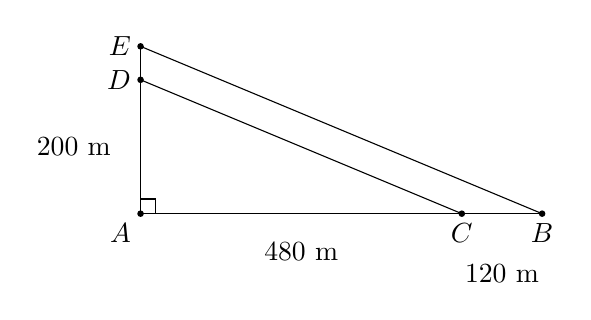
\begin{tikzpicture}[scale=0.85]
  \coordinate (A) at (0, 0);
  \coordinate (C) at (4.8, 0);
  \coordinate (B) at (6, 0);
  \coordinate (D) at (0, 2);
  \coordinate (E) at (0, 2.5);
  \draw (A) -- (B);
  \draw (A) -- (E);
  \draw (C) -- (D);
  \draw (B) -- (E);
  \draw (0.22, 0) -- (0.22, 0.22) -- (0, 0.22);
  \foreach \p in {A, C, B, D, E} \fill (\p) circle (1.4pt);
  \node[below left]  at (A) {$A$};
  \node[below] at (C) {$C$};
  \node[below] at (B) {$B$};
  \node[left]  at (D) {$D$};
  \node[left]  at (E) {$E$};
  \node[below] at (2.4, -0.28) {$480$ m};
  \node[below] at (5.4, -0.62) {$120$ m};
  \node[left]  at (-0.3, 1) {$200$ m};
\end{tikzpicture}
